\documentclass{article}
\usepackage{graphicx} % Required for inserting images
\usepackage[margin=2.5cm]{geometry}
\usepackage[T1]{fontenc}
\usepackage{lmodern}
\usepackage{amsmath}
\usepackage{booktabs}
\usepackage{caption}
\usepackage[numbers,sort&compress]{natbib}
\usepackage[hidelinks]{hyperref}

\graphicspath{{figures/}{./}}

\title{HealthMonitoring}
\author{Manideepa Mukherjee Bhakat}
\date{October 2026}

\begin{document}
\maketitle

\begin{center}
{\Large\textbf{BodySync: Comparing a Sync Score and a Personal-Normal Score on Wrist Physiology}}\\[4pt]
{\large Progress report: free-living data and laboratory stress datasets}
\end{center}

\begin{abstract}
Wrist wearables record heart rate, electrodermal activity (EDA) and skin temperature continuously. We compare two candidate scores built from these signals. Score~A (\emph{sync}) measures whether the three signals move together the way they usually do for a person. Score~B (\emph{BodySync}) measures how far their levels are from the person's own normal for the same situation, counting only changes in the stress direction. Both were built on ZU-PWD~'25, a free-living Empatica EmbracePlus dataset (27 people, 901{,}440 minutes). In ZU-PWD, coupling features were close to chance at telling sleep, rest and activity apart (balanced accuracy 0.37, vs.\ 0.81 for signal levels). On four public laboratory stress datasets recorded with the Empatica E4, the sync score did not separate stress from calm in any fair test (within-person AUC 0.46--0.49). BodySync separated acute stress on WESAD (AUC 0.78, lower under stress for 12 of 15 people) and more weakly on two other laboratory datasets (AUC 0.60 and 0.54). Testing on everyday-life stress datasets is the next step.
\end{abstract}

\section{Introduction}

Sun et al.~\cite{sun2026trust} showed that EDA, heart-rate variability and skin temperature change when people read health information, and predicted trust from these signals. Their signals were analysed separately, in a single laboratory session, and the authors call for longitudinal, ecological studies. Our starting idea (\emph{BodySync}) was to look at the relationships between signals instead: when the body is in a familiar state its signals should move together in a familiar way, and a break in that pattern (a \emph{desync}) might mark stress, illness or poor sleep. Network physiology supports the idea that coupling between organ systems changes with state~\cite{bashan2012network}, and coupling features have improved emotion recognition in the laboratory~\cite{valenza2013coupling}.

The dataset we started from, ZU-PWD~'25~\cite{evangelista2025zupwd}, already has a wellness score: the Physiological Wellness Index~\cite{sharma2025pwi}, a hand-weighted average of signal levels. It was checked on a few example days only, and the free copy of the dataset has no stress labels. In this report we (i) test whether coupling adds information over signal levels on ZU-PWD, (ii) define two candidate scores, sync (A) and a personal-normal score (B), and (iii) compare them on public laboratory stress datasets recorded with the same family of wristband.

\section{Data}

\paragraph{ZU-PWD~'25.} Twenty-seven people wore an Empatica EmbracePlus in daily life between March 2024 and May 2025. The free copy has 901{,}440 one-minute rows with 24 columns, including pulse rate, EDA, skin temperature, sleep stage and activity intensity. After removing minutes when the watch was not worn (wear detection $<$50\%) and implausible values (heart rate outside 35--200~bpm, temperature outside 25--40\,$^\circ$C), 484{,}636 minutes had all three signals. Each minute was labelled \emph{asleep} (sleep stage 101), \emph{resting} (awake and sedentary), \emph{active} (awake, moderate or vigorous activity) or \emph{other}. These labels come from Empatica's own accelerometer-based algorithms. Heart-rate variability and breathing rate are mostly recorded only when the wrist is still, so we used heart rate, EDA and temperature.

\paragraph{Public stress datasets.} Table~\ref{tab:datasets} lists the public Empatica E4 datasets with stress labels that we use. The E4 is the predecessor of the EmbracePlus and records the same three signals at a higher rate. This report covers the four laboratory datasets. The three everyday-life datasets are prepared and are the next step. Each dataset was converted to a common format of 2-minute windows sliding by 30~s.

\begin{table}[htbp]
\centering
\caption{Public Empatica E4 datasets with stress labels. Citations from OpenAlex, November 2026.}
\label{tab:datasets}
\footnotesize
\begin{tabular}{llrlrl}
\toprule
Dataset & Paper & Cites & Setting & People & Stress label \\
\midrule
WESAD & Schmidt 2018~\cite{schmidt2018wesad} & 1{,}352 & lab & 15 & Trier Social Stress Test \\
Stress-Predict & Iqbal 2022~\cite{iqbal2022stresspredict} & 113 & lab & 35 & Stroop test, interview \\
Stress + exercise & Hongn 2025~\cite{hongn2025stress} & 37 & lab & 36 & arithmetic/emotional tasks \\
EmpaticaE4Stress & Campanella 2024~\cite{campanella2024e4stress} & 26 & lab & 29 & timed puzzle tasks \\
\midrule
\multicolumn{6}{l}{\emph{Next step: everyday-life datasets}} \\
Nurse stress & Hosseini 2022~\cite{hosseini2022nurse} & 119 & hospital & 15 & nurse-rated stress \\
ADARP & Sah 2022~\cite{sah2022adarp} & 13 & daily life & 11 & button press when stressed \\
CAN-STRESS & Rahimi Azghan 2025~\cite{azghan2025canstress} & 1 & daily life & 62 & stress ratings 0--9 \\
\bottomrule
\end{tabular}
\end{table}

\begin{figure}[htbp]
\centering
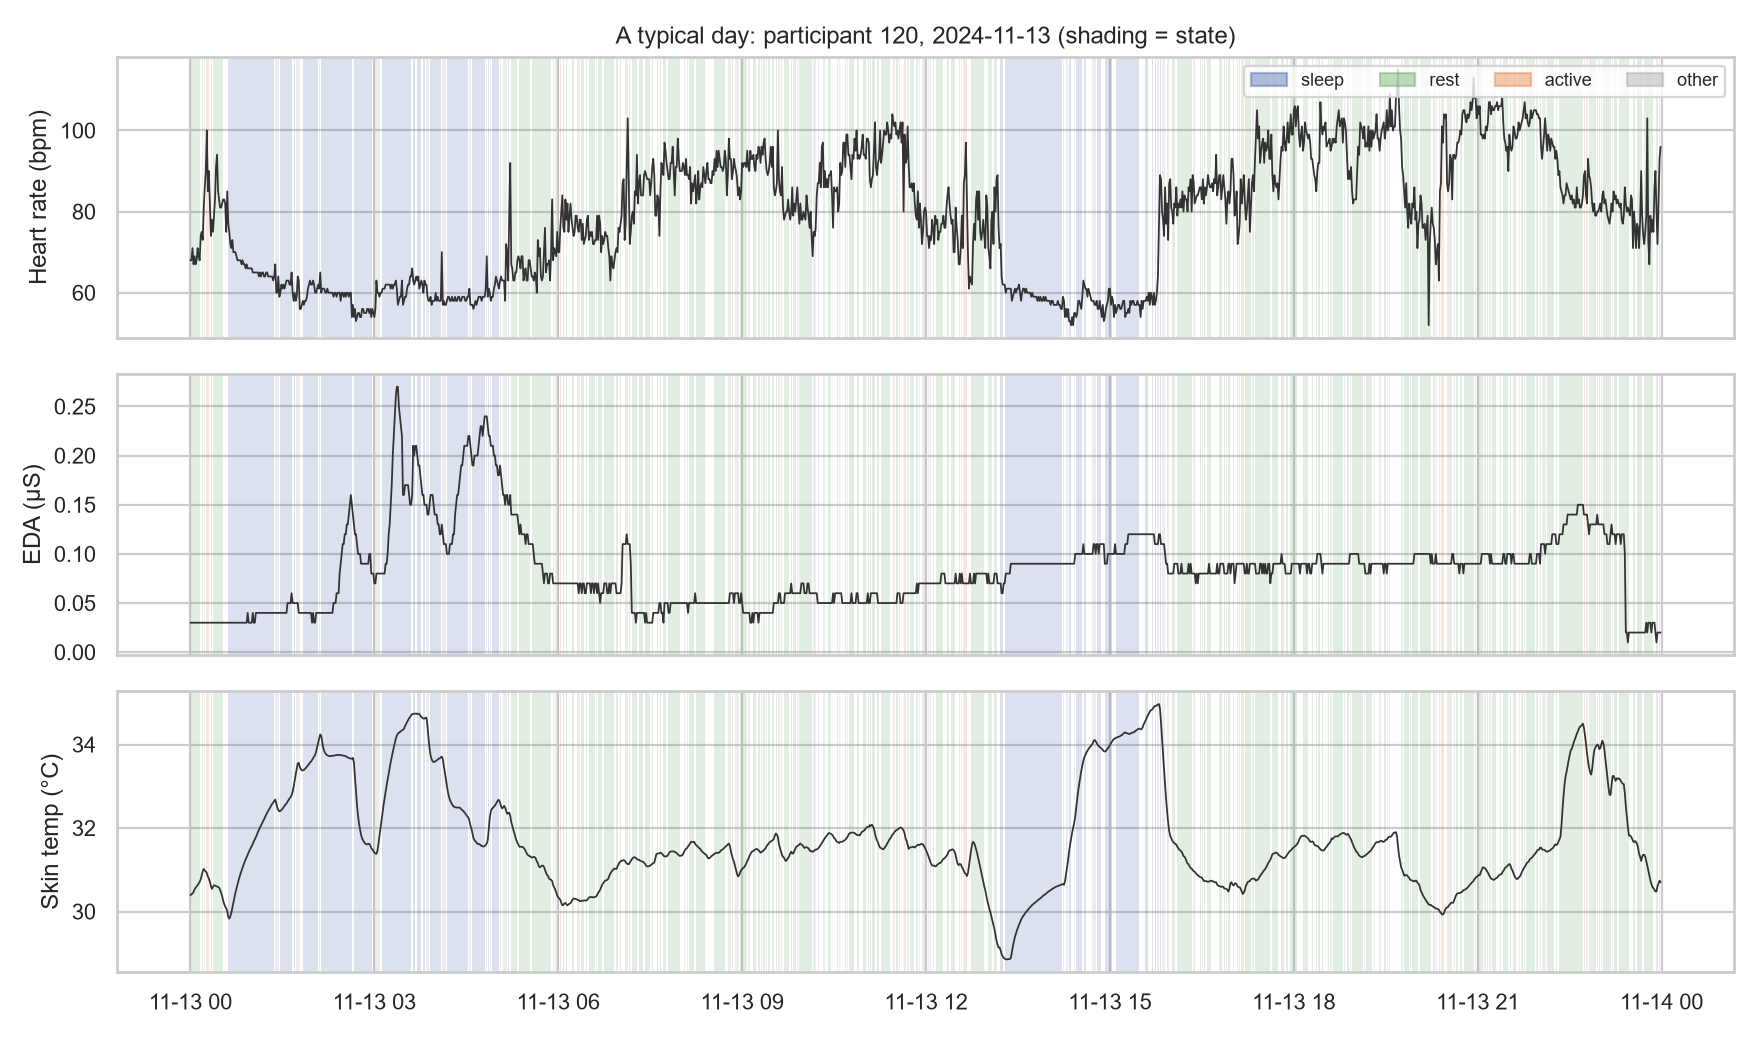
\includegraphics[width=0.95\linewidth]{fig1_typical_day.png}
\caption{One day of ZU-PWD data for one participant. Shading shows the watch's state label.}
\label{fig:day}
\end{figure}

\section{Methods}

\subsection{Windows and features (ZU-PWD)}
Each person's timeline was cut into 30-minute windows sliding by 15 minutes. A window was given a state only if at least 70\% of its minutes shared it; otherwise it was \emph{other}. Windows needed at least 75\% of minutes with all three signals. \emph{Level} features were the mean and standard deviation of each signal. \emph{Personal} features were each mean relative to the person's own median and interquartile range. \emph{Coupling} features were the Pearson correlation of each signal pair (HR--EDA, HR--temperature, EDA--temperature), on raw values and on minute-to-minute changes.

\subsection{Does coupling add information?}
XGBoost classified windows as sleep, rest or active, and separately sleep vs.\ rest (both still, so movement cannot separate them). Each person was tested on a model trained on the others (leave-one-subject-out). Per-person balanced accuracy was compared between feature sets with a paired Wilcoxon test.

\subsection{The two scores}
Both scores use the same steps on different inputs:
\begin{enumerate}
\item For each person and situation, the \emph{normal} is the median of each input across that person's windows in that situation, and the typical spread is the scaled median absolute deviation. Situations with fewer than 10 windows fall back to the person's overall normal.
\item Each input becomes a number of typical spreads away from normal, $z$; the distance is the root mean square of the $z$ values.
\item The score is $100 / (1 + d/2)$, so the normal scores 100 and two spreads away scores 50.
\end{enumerate}
\textbf{Score A (sync)} uses the three pairwise correlations as inputs, and any deviation counts. \textbf{Score B (BodySync)} uses mean heart rate, log EDA and mean skin temperature, and only deviations in the stress direction count (heart rate up, EDA up, temperature down). The input furthest from normal is reported as the reason for a low score. In ZU-PWD the situation is the watch's state label. In the laboratory datasets the normal is the baseline rest period.

\subsection{Evaluation}
For each dataset and score we report the within-person AUC: how well a lower score separates a person's stress windows from their calm windows, averaged over people (0.5 = chance). We also report how many people scored lower under stress, with a paired Wilcoxon test. To avoid an unfair advantage, stress was compared with \emph{later} rest, amusement or meditation, never with the baseline that set the normal. EmpaticaE4Stress has no later rest, so it is the one exception and is marked as a weaker test.

\section{Results}

\subsection{Coupling vs.\ levels on ZU-PWD}
Coupling features alone were close to chance (Table~\ref{tab:coupling}). Adding them to level and personal features raised balanced accuracy by less than one percentage point. That gain was detectable for the three-class task but not for sleep vs.\ rest (Table~\ref{tab:coupling_paired}). The correlations themselves overlapped almost completely across states (Figure~\ref{fig:coupling}).

\begin{table}[htbp]
\centering
\caption{Leave-one-subject-out balanced accuracy on ZU-PWD (chance: 0.33 and 0.50).}
\label{tab:coupling}
\begin{tabular}{lcc}
\toprule
Features & Sleep / rest / active & Sleep vs rest \\
\midrule
Coupling only & 0.372 & 0.562 \\
Levels & 0.807 & 0.831 \\
Levels + personal & 0.825 & 0.878 \\
Levels + personal + coupling & 0.835 & 0.884 \\
\bottomrule
\end{tabular}
\end{table}

\begin{table}[htbp]
\centering
\caption{Per-person paired comparisons (Wilcoxon signed-rank test).}
\label{tab:coupling_paired}
\small
\begin{tabular}{llccc}
\toprule
Task & Comparison & Median gain & People better & $p$ \\
\midrule
Sleep / rest / active & levels + personal + coupling vs levels + personal & +0.006 & 13/20 & 0.006 \\
Sleep / rest / active & coupling only vs levels & -0.397 & 0/20 & $<$0.001 \\
Sleep vs rest & levels + personal + coupling vs levels + personal & +0.003 & 10/18 & 0.326 \\
Sleep vs rest & coupling only vs levels & -0.286 & 0/18 & $<$0.001 \\
\bottomrule
\end{tabular}
\end{table}

\begin{figure}[htbp]
\centering
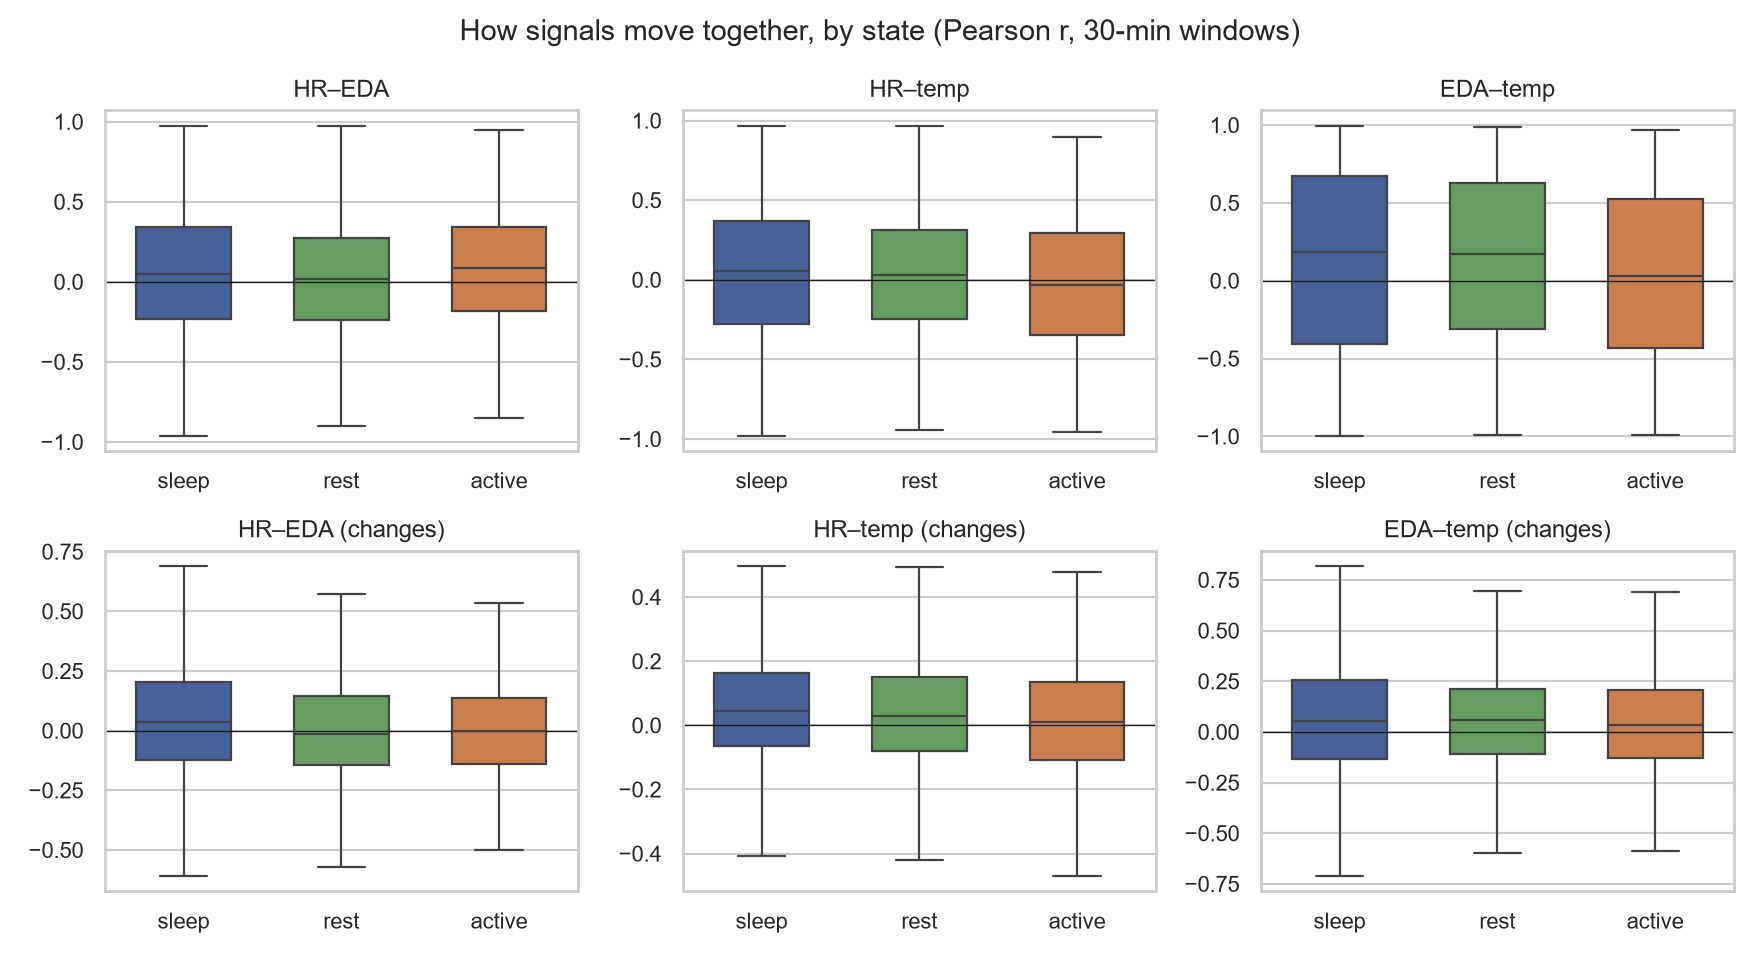
\includegraphics[width=0.85\linewidth]{fig2_coupling_by_state.png}
\caption{Pairwise correlations in 30-minute windows by state. The distributions overlap almost completely.}
\label{fig:coupling}
\end{figure}

\subsection{Sync vs.\ BodySync on the laboratory stress datasets}
Table~\ref{tab:results} shows the comparison. On every fair test the sync score was at chance (AUC 0.46--0.49), including on WESAD. BodySync separated stress clearly on WESAD (AUC 0.78; lower under stress for 12 of 15 people) and more weakly on the stress + exercise dataset (AUC 0.60) and on Stress-Predict (AUC 0.54). Both scores were high on EmpaticaE4Stress, but that test compares stress with the baseline that defined the normal, so it overstates performance. When BodySync dropped under stress, the most common reason given was high EDA.

\begin{table}[htbp]
\centering
\caption{Stress vs.\ calm for both scores on the laboratory datasets. AUC: within-person AUC averaged over people. Lower: people whose mean score was lower under stress. Bold: the higher AUC of the two scores. $^\dagger$Weaker test (stress vs.\ the baseline that set the normal).}
\label{tab:results}
\resizebox{\linewidth}{!}{\begin{tabular}{llccccccc}
\toprule
 & & & \multicolumn{3}{c}{A: sync} & \multicolumn{3}{c}{B: BodySync} \\
\cmidrule(lr){4-6}\cmidrule(lr){7-9}
Dataset & Setting & $n$ & AUC & Lower & $p$ & AUC & Lower & $p$ \\
\midrule
WESAD & lab & 15 & 0.46 & 6/15 & 0.359 & \textbf{0.78} & 12/15 & 0.004 \\
Stress-Predict & lab & 35 & 0.48 & 15/35 & 0.501 & \textbf{0.54} & 19/35 & 0.342 \\
Stress + exercise & lab & 35 & 0.49 & 16/35 & 0.554 & \textbf{0.60} & 21/35 & 0.016 \\
EmpaticaE4Stress$^\dagger$ & lab & 29 & 0.90 & 29/29 & $<$0.001 & \textbf{0.92} & 28/29 & $<$0.001 \\
\bottomrule
\end{tabular}}
\end{table}

\begin{figure}[htbp]
\centering
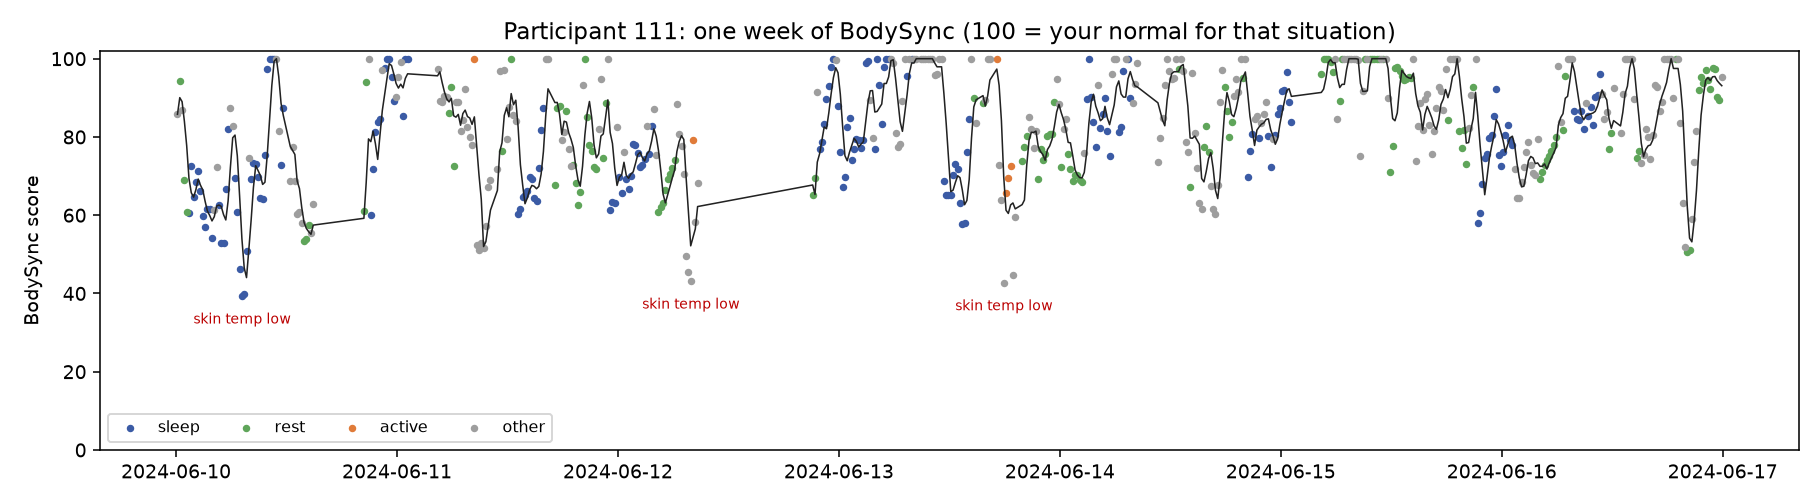
\includegraphics[width=\linewidth]{fig3_example_week.png}
\caption{What BodySync looks like on ZU-PWD: one week of scores for one participant, with the reason given for the three lowest points.}
\label{fig:week}
\end{figure}

\section{Discussion}

The original BodySync idea, that a break in how signals move together marks stress, was not supported so far. Coupling barely differed between sleep, rest and activity in free-living data, and the sync score was at chance on every fair laboratory stress test. This agrees with Xu et al.~\cite{xu2026pilot}, who found that correlation features from consumer wearables did not beat EDA alone. Laboratory work that found coupling useful used ECG and respiration belts at much higher resolution~\cite{valenza2013coupling}. We found no benefit even on WESAD at one sample per second, so the problem is not only ZU-PWD's one-minute resolution.

Signal levels compared with a personal normal carried most of the information. BodySync picked up the strong, acute response to the Trier Social Stress Test, mainly through rising EDA, and weaker responses in the other laboratory protocols. Using a separate normal per situation (asleep, resting, active) is meant to keep exercise from looking like stress, a known weakness of context-free wrist stress detection~\cite{gjoreski2017context}.

\paragraph{Limitations.}
\begin{itemize}
\item \textbf{Retrospective normal:} each person's normal is computed from their whole recording. A deployed version needs a calibration period or a past-only, rolling normal.
\item \textbf{No drift handling:} the normal is fixed, so slow changes are not adjusted for.
\item \textbf{State labels:} ZU-PWD states come from Empatica's algorithms, not ground truth, and the free copy has no stress labels.
\item \textbf{Sample:} the laboratory datasets have 15--36 people each.
\end{itemize}

\section{Next steps}
\begin{itemize}
\item Run both scores on the three everyday-life datasets (nurse stress, ADARP, CAN-STRESS), where stress is self-reported.
\item Check BodySync on ZU-PWD against what the watch records: exercise periods and sleep quality.
\item Replace the retrospective normal with a past-only one.
\end{itemize}

\paragraph{Code.} \url{https://github.com/swaylakh/bodysync}

\begin{thebibliography}{15}
\providecommand{\natexlab}[1]{#1}
\providecommand{\url}[1]{\texttt{#1}}
\expandafter\ifx\csname urlstyle\endcsname\relax
  \providecommand{\doi}[1]{doi: #1}\else
  \providecommand{\doi}{doi: \begingroup \urlstyle{rm}\Url}\fi

\bibitem[Sun et~al.(2026)Sun, Ma, Wei, Cesar, Bosch, and El~Ali]{sun2026trust}
Xin Sun, Rongjun Ma, Shu Wei, Pablo Cesar, Jos~A. Bosch, and Abdallah El~Ali.
\newblock Understanding trust toward human versus {AI}-generated health
  information through behavioral and physiological sensing.
\newblock \emph{International Journal of Human-Computer Studies}, 209:\penalty0
  103714, 2026.
\newblock \doi{10.1016/j.ijhcs.2025.103714}.

\bibitem[Bashan et~al.(2012)Bashan, Bartsch, Kantelhardt, Havlin, and
  Ivanov]{bashan2012network}
Amir Bashan, Ronny~P. Bartsch, Jan~W. Kantelhardt, Shlomo Havlin, and
  Plamen~Ch. Ivanov.
\newblock Network physiology reveals relations between network topology and
  physiological function.
\newblock \emph{Nature Communications}, 3:\penalty0 702, 2012.
\newblock \doi{10.1038/ncomms1705}.

\bibitem[Valenza et~al.(2013)Valenza, Lanat{\`a}, and
  Scilingo]{valenza2013coupling}
Gaetano Valenza, Antonio Lanat{\`a}, and Enzo~Pasquale Scilingo.
\newblock Improving emotion recognition systems by embedding cardiorespiratory
  coupling.
\newblock \emph{Physiological Measurement}, 34\penalty0 (4):\penalty0 449--464,
  2013.
\newblock \doi{10.1088/0967-3334/34/4/449}.

\bibitem[Evangelista et~al.(2025)Evangelista, Nazir, Bukhari, Dahmani,
  Tbaishat, and Sharma]{evangelista2025zupwd}
Evangelista, Nazir, Bukhari, Dahmani, Tbaishat, and Sharma.
\newblock Zayed university physiological wellness dataset 2025 ({ZU-PWD} '25).
\newblock IEEE DataPort, 2025.

\bibitem[Sharma et~al.(2025)Sharma, Ghista, Evangelista, Bukhari, Meena, and
  Thakur]{sharma2025pwi}
Sharma, Ghista, Evangelista, Bukhari, Meena, and Thakur.
\newblock Introducing a physiological wellness index ({PWI}) for health and
  well-being.
\newblock \emph{IADIS International Journal on Computer Science and Information
  Systems}, 20\penalty0 (2):\penalty0 19--48, 2025.
\newblock \doi{10.33965/ijcsis_2025200202}.

\bibitem[Schmidt et~al.(2018)Schmidt, Reiss, D{\"u}richen, Marberger, and
  Van~Laerhoven]{schmidt2018wesad}
Philip Schmidt, Attila Reiss, Robert D{\"u}richen, Claus Marberger, and Kristof
  Van~Laerhoven.
\newblock Introducing {WESAD}, a multimodal dataset for wearable stress and
  affect detection.
\newblock In \emph{Proceedings of the 20th ACM International Conference on
  Multimodal Interaction}, pages 400--408, 2018.
\newblock \doi{10.1145/3242969.3242985}.

\bibitem[Hosseini et~al.(2022)Hosseini, Gottumukkala, Katragadda, Bhupatiraju,
  Ashkar, Borst, et~al.]{hosseini2022nurse}
Seyedmajid Hosseini, Raju Gottumukkala, Satya Katragadda, Ravi~Teja
  Bhupatiraju, Ziad Ashkar, Christoph~W. Borst, et~al.
\newblock A multimodal sensor dataset for continuous stress detection of nurses
  in a hospital.
\newblock \emph{Scientific Data}, 9:\penalty0 255, 2022.
\newblock \doi{10.1038/s41597-022-01361-y}.

\bibitem[Iqbal et~al.(2022)Iqbal, Simpkin, Roshan, Glynn, Killilea, Walsh,
  et~al.]{iqbal2022stresspredict}
Talha Iqbal, Andrew~J. Simpkin, Davood Roshan, Nicola Glynn, John Killilea,
  Jane~C. Walsh, et~al.
\newblock Stress monitoring using wearable sensors: A pilot study and
  {Stress-Predict} dataset.
\newblock \emph{Sensors}, 22\penalty0 (21):\penalty0 8135, 2022.
\newblock \doi{10.3390/s22218135}.

\bibitem[Hongn et~al.(2025)Hongn, Bosch, Prado, Ferr{\'a}ndez~Vicente, and
  Bonomini]{hongn2025stress}
Andrea Hongn, Facundo Bosch, Lara~Eleonora Prado, Jos{\'e}~Manuel
  Ferr{\'a}ndez~Vicente, and Mar{\'i}a~Paula Bonomini.
\newblock Wearable physiological signals under acute stress and exercise
  conditions.
\newblock \emph{Scientific Data}, 12:\penalty0 520, 2025.
\newblock \doi{10.1038/s41597-025-04845-9}.

\bibitem[Campanella et~al.(2024)Campanella, Altaleb, Belli, Pierleoni, and
  Palma]{campanella2024e4stress}
Sara Campanella, Ayham Altaleb, Alberto Belli, Paola Pierleoni, and Lorenzo
  Palma.
\newblock {PPG} and {EDA} dataset collected with {Empatica E4} for stress
  assessment.
\newblock \emph{Data in Brief}, 53:\penalty0 110102, 2024.
\newblock \doi{10.1016/j.dib.2024.110102}.

\bibitem[Sah et~al.(2022)Sah, McDonell, Pendry, Parent, Ghasemzadeh, and
  Cleveland]{sah2022adarp}
Ramesh~Kumar Sah, Michael~G. McDonell, Patricia Pendry, Sara~C. Parent, Hassan
  Ghasemzadeh, and Michael~John Cleveland.
\newblock {ADARP}: A multi modal dataset for stress and alcohol relapse
  quantification in real life setting.
\newblock In \emph{IEEE International Conference on Wearable and Implantable
  Body Sensor Networks (BSN)}, pages 1--4, 2022.
\newblock \doi{10.1109/BSN56160.2022.9928495}.

\bibitem[Rahimi~Azghan et~al.(2025)Rahimi~Azghan, Glodosky, Sah, Cuttler,
  McLaughlin, Cleveland, et~al.]{azghan2025canstress}
Reza Rahimi~Azghan, Nicholas~C. Glodosky, Ramesh~Kumar Sah, Carrie Cuttler,
  Ryan~J. McLaughlin, Michael~John Cleveland, et~al.
\newblock {CAN-STRESS}: A real-world multimodal dataset for understanding
  cannabis use, stress, and physiological responses.
\newblock In \emph{IEEE International Conference on Wearable and Implantable
  Body Sensor Networks (BSN)}, pages 1--4, 2025.
\newblock \doi{10.1109/BSN66969.2025.11337465}.

\bibitem[Xu et~al.(2026)Xu, Cao, Barnett-Cowan, Irving, Niechwiej-Szwedo,
  Kearns, et~al.]{xu2026pilot}
Rongbing Xu, Shi~Chao Cao, Michael Barnett-Cowan, Elizabeth~L. Irving, Ewa
  Niechwiej-Szwedo, Suzanne~K. Kearns, et~al.
\newblock Consumer-grade wearable sensors for classifying pilot workload and
  stress during real flight training: A leave-one-subject-out validation study.
\newblock \emph{Sensors}, 26\penalty0 (12):\penalty0 3627, 2026.
\newblock \doi{10.3390/s26123627}.

\bibitem[Gjoreski et~al.(2017)Gjoreski, Lu{\v{s}}trek, Gams, and
  Gjoreski]{gjoreski2017context}
Martin Gjoreski, Mitja Lu{\v{s}}trek, Matja{\v{z}} Gams, and Hristijan
  Gjoreski.
\newblock Monitoring stress with a wrist device using context.
\newblock \emph{Journal of Biomedical Informatics}, 73:\penalty0 159--170,
  2017.
\newblock \doi{10.1016/j.jbi.2017.08.006}.

\end{thebibliography}

\end{document}
